%Definiciones previas y uso de paqueterías
\documentclass[12pt]{article}
\usepackage[utf8]{inputenc}
\usepackage{graphicx} % Required for inserting images
\usepackage[spanish]{babel}
\usepackage{geometry}
\usepackage{setspace}
\usepackage{sectsty} %Para cambiar el tamaño de diferentes secciones

%Para el formato APA
\usepackage{apacite}

%Márgenes
\newgeometry{left=1in, right=1in, top=1in, bottom=1in}

\begin{document}

%Haciendo portada
\begin{titlepage}
\centering
{
\includegraphics[width=0.35\textwidth]{img/Screenshot from 2025-07-01 09-12-19.png}\par}
\vspace{0.5cm}
{\bfseries\Large Universidad Nacional Mayor de San Marcos\par}
{\large Universidad del Perú, Decana de América\par}
{\scshape\Large Facultad de Ingeniería de Sistemas e Informatica\par}
{\scshape\Large Escuela Profesional de Ingeniería de Sistemas\par}
\vspace{0.5cm}
{\bfseries\large Informe Proyecto Final

Verificador de acceso mediante código QR y reconocimiento facial\par}
\vspace{0.05cm}
{\bfseries\large Grupo N.º 8\par}
\vspace{0.5cm}

{\bfseries\large Asigntatura:}
{\large Programación de Computadoras I\par}
\vspace{0.5cm}

{\bfseries\large Docente:}
{\large Guerra Grados, Luis Angel\par}
\vspace{0.5cm}

{\bfseries\large Integrantes:\par}
{\large
\begin{center}
\begin{tabular}{c@{\hspace{2cm}}c}
Cardenas Huaman, Ariana Milagros & 24200093 \\
Cruz Ramos, Alysson Kiara    	& 24200143 \\
Flores Hoyos, Mathias Pavel Diego & 24200014 \\
Meza Dalguer, Anyel Giuliana 	& 24200111 \\
\end{tabular}
\end{center}}

\vspace{1in}

{\bfseries\large Lima, Perú\par}
{\bfseries\large 2025-I\par}
\end{titlepage}
%Fin de portada

%Cuerpo del documento
	%Tamaño de fuente 12 e interlineado 1.5
{\fontsize{12}{18}\selectfont % Fuente 12pt, interlineado 1.5x
\doublespacing
    
% Cambiar tamaño de títulos para que escalen con 12pt
\sectionfont{\Large} 	% Sección: tamaño Large (aprox 14.4pt)
\subsectionfont{\large} % Subsección: tamaño large (12pt)
\subsubsectionfont{\normalsize}

%Índice
\tableofcontents{}

%Introducción
\section{Introducción}
La identificación facial automatizada ha transformado significativamente la manera en que se diseñan y utilizan los sistemas tecnológicos orientados a la seguridad, ofreciendo soluciones eficientes y adaptables a distintos contextos. En este proyecto se desarrolla un sistema de reconocimiento facial utilizando el lenguaje de programación Python, con un enfoque centrado en el entrenamiento de algoritmos capaces de identificar patrones biométricos únicos en cada individuo. Mediante técnicas de aprendizaje automático, el sistema es capaz de procesar imágenes faciales, extraer características relevantes y convertirlas en estructuras matemáticas que permiten realizar comparaciones precisas de forma ágil.

Como parte del flujo de autenticación, se incorpora una fase previa basada en la lectura de un código QR, el cual cumple la función de habilitar el acceso al sistema. Este código, generado de manera personalizada contiene su código de estudiante. Al escanearse, el sistema desbloquea la funcionalidad de verificación facial, activando automáticamente la cámara del dispositivo para iniciar la detección y análisis del rostro para corroborar la información ingresada anteriormente.

En cuanto al procesamiento de imágenes, se han priorizado técnicas que equilibran eficiencia y precisión. Por ejemplo, la conversión a escala de grises se implementa como una medida de optimización que reduce la carga computacional sin sacrificar la calidad del reconocimiento. Este enfoque técnico permite mantener un desempeño constante incluso en entornos con recursos limitados. Si bien el sistema presenta ciertos desafíos, como la sensibilidad a condiciones de iluminación adversa o la necesidad de una posición frontal del rostro, los resultados obtenidos demuestran su viabilidad dentro de escenarios controlados. El desarrollo abarca desde la recopilación de datos hasta la implementación funcional del modelo, evidenciando el potencial real de la inteligencia artificial aplicada en entornos académicos para mejorar procesos de autenticación e ingreso.

%Planteamiento del problema
\section{Planteamiento del problema y justificación}
En el contexto de la Universidad Nacional Mayor de San Marcos, existe una problemática significativa en el control de accesos que afecta tanto la seguridad como la eficiencia institucional. El sistema actual, basado en identificación mediante carnets físicos, presenta múltiples limitaciones que comprometen la integridad de las instalaciones y la agilidad operativa. Simultáneamente, los procesos manuales de verificación ocasionan congestiones en los accesos principales, particularmente durante horas de alta circulación de personas, retrasando la movilidad de estudiantes y docentes hacia sus actividades académicas.Esta situación demanda urgentemente una solución tecnológica que modernice los procesos de identificación, garantizando simultáneamente mayor seguridad y eficiencia operativa.

La implementación de un sistema de reconocimiento facial se presenta como la alternativa óptima para superar estos desafíos. Esta innovación reforzaría sustancialmente la seguridad institucional al eliminar los riesgos de suplantación asociados a documentos físicos, mediante la verificación biométrica en tiempo real contra una base de datos centralizada. La tecnología permitiría agilizar significativamente los flujos de acceso, eliminando cuellos de botella en los puntos de ingreso y facilitando el registro automático de asistencia con fines académicos y estadísticos.

Desde la perspectiva ambiental, el proyecto promovería la sostenibilidad al reducir el consumo de materiales plásticos y papel utilizados en la producción de carnets físicos o fichas de asistencia. Los usuarios se beneficiarían en comodidad y autonomía al liberarse de la necesidad de portar documentos físicos, eliminando los problemas asociados a su pérdida u olvido. La solución está diseñada con capacidad de escalamiento, permitiendo su adaptación a diversos escenarios institucionales más allá del ámbito universitario, incluyendo colegios, centros médicos y empresas privadas que requieran sistemas de control de acceso seguros y eficientes.

Esta iniciativa no solo modernizaría la gestión de accesos en la UNMSM, sino que establecería un precedente tecnológico para otras instituciones educativas nacionales. Al implementar un sistema biométrico de vanguardia, la universidad reforzaría su posición como institución líder en innovación tecnológica, al tiempo que contribuiría a la transformación digital del país con un modelo sostenible, seguro y eficiente.

%Objetivos
\section{Objetivos}
\subsection{Objetivo General}
Desarrollar e implementar un sistema de reconocimiento facial para el control de acceso en las instalaciones de la Universidad Nacional Mayor de San Marcos, que mejore la seguridad institucional, optimice los procesos de ingreso y sustituya los métodos tradicionales de identificación física, contribuyendo a la modernización tecnológica de la universidad.

\subsection{Objetivos Específicos}
Automatizar los procesos de control de acceso y registro de asistencia, eliminando la dependencia de carnets físicos y reduciendo los tiempos de verificación en los puntos de ingreso principales, con capacidad de generar reportes automatizados para la gestión administrativa.

Diseñar una solución escalable y adaptable que pueda extenderse a diferentes facultades y dependencias de la universidad, con potencial para ser implementado en otras instituciones educativas o centros que requieran sistemas de control de acceso seguros y eficientes.

%Marco Teórico
\section{Marco Teórico}
\subsection{Procesamiento de Imágenes}
El reconocimiento facial automatizado requiere un pre procesamiento eficiente de imágenes para mejorar la velocidad del sistema sin sacrificar precisión. Un paso fundamental es la conversión a escala de grises, que elimina la información de color redundante y reduce la complejidad computacional al trabajar con matrices de un solo canal (Almeida and Silva, 2021).

Asimismo, el redimensionamiento uniforme de las imágenes (por ejemplo, 200×200 píxeles) asegura la homogeneidad en la entrada del modelo, facilitando los cálculos durante el entrenamiento y reconocimiento facial (Sharma et al., 2019).

\subsection{Detección Facial con Haar Cascade}
El método Haar Cascade, desarrollado por Viola y Jones (2001), es una técnica ampliamente utilizada para la detección de objetos. Este clasificador utiliza características Haar y el algoritmo Adaboost para seleccionar y optimizar las características más relevantes, ejecutando una cascada de clasificadores que mejora la precisión y reduce los falsos positivos. En Python, esta técnica se implementa mediante la función cv2.CascadeClassifier de OpenCV (Kumar and Raj, 2022).

Las ventajas de Haar Cascade incluyen su baja demanda de cómputo y alta velocidad, lo que lo hace ideal para aplicaciones en tiempo real, especialmente en dispositivos de recursos limitados.

\subsection{Reconocimiento Facial con LBPH (Local Binary Patterns Histograms)}
El algoritmo LBPH es uno de los métodos más eficaces y robustos para el reconocimiento facial en ambientes reales. A diferencia de Eigenfaces o Fisherfaces, que se basan en técnicas de reducción de dimensionalidad como PCA, el LBPH opera describiendo localmente la textura de una imagen mediante patrones binarios, ofreciendo mayor tolerancia a cambios en iluminación o expresiones faciales (Ahonen et al., 2006).

Este método divide la imagen facial en una cuadrícula, calcula un histograma de patrones binarios locales (LBP) en cada celda, y concatena esos histogramas para formar un vector característico. Estos vectores se comparan con los almacenados en la fase de entrenamiento utilizando una métrica de distancia, generalmente la distancia Euclidiana. En Python, la librería OpenCV permite implementar este modelo de manera directa con cv2.face.LBPHFaceRecognizer\_create().

\subsection{Optimización y Precisión}
El uso del PCA en reconocimiento facial no solo mejora la velocidad de procesamiento, sino también la precisión, siempre que se elijan adecuadamente los componentes principales que retienen mayor varianza (Zhao et al., 2020). Se ha demostrado que una adecuada reducción de dimensionalidad puede acelerar el sistema sin afectar significativamente su tasa de aciertos, especialmente en bases de datos de tamaño medio.

\subsection{Programación en Python con OpenCV}
La librería OpenCV (Open Source Computer Vision Library) proporciona una interfaz de alto nivel para procesamiento de imágenes en Python. Entre sus funciones más relevantes se encuentran:
\begin{itemize}
    {\bfseries\item cv2.VideoCapture:} captura video desde una fuente (archivo o webcam).
    {\bfseries\item cv2.cvtColor:} convierte imágenes a escala de grises.
    {\bfseries\item cv2.resize:} ajusta dimensiones de imagen.
    {\bfseries\item CascadeClassifier.detectMultiScale:} detecta rostros en una imagen. (Metev, 2008; Khan et al., 2019).
\end{itemize}

La arquitectura modular del sistema permite escalar el proyecto fácilmente, integrándolo a distintas interfaces o bases de datos, haciendo uso del paradigma de programación estructurada y funciones encapsuladas.

%Metodología
\section{Metodología}
El sistema de reconocimiento facial y gestión de alumnos se desarrolló bajo una metodología estructurada que combina técnicas de programación modular con algoritmos de visión por computadora. El diseño se centró en tres pilares fundamentales: la identificación mediante códigos QR, el reconocimiento facial basado en el algoritmo LBPH y la gestión centralizada de datos a través de un archivo CSV.

A continuación, se describen las etapas clave de este proceso:

\subsection{Interfaz de usuario}
La interfaz de usuario del sistema está diseñada para ser intuitiva y funcional, dividiéndose en tres módulos principales: Acceso de Alumnos, Registro de Nuevos Alumnos y Panel de Administración. A continuación, se detalla la metodología empleada en su desarrollo.

\subsection{Acceso de Alumnos (Opción 1. Acceder)}
El módulo de acceso implementa un sistema de verificación en dos etapas que combina identificación por código QR con reconocimiento facial. Todo el proceso de autenticación se completa en menos de 5 segundos, garantizando tanto seguridad como eficiencia operativa.

\begin{itemize}
	{\bfseries\item Validación del código QR:\par}
    {\normalsize El alumno presenta un código QR que contiene su código de estudiante, continuamente el sistema verifica que este código exista en la base de datos registrada.}

    {\bfseries\item Reconocimiento facial:\par}
    {\normalsize Si el código es válido, se activa la cámara para verificar el rostro del alumno, a través del algoritmo LBPH (Local Binary Patterns Histograms), el sistema compara los rasgos faciales con el modelo previamente almacenado. Si la coincidencia es exitosa, se concede el acceso; de lo contrario, se deniega.}
\end{itemize}
Este proceso asegura que solo los alumnos registrados y debidamente identificados puedan ingresar al sistema.

\subsection{Registro de Nuevos Alumnos (Opción 2. Registrar alumno )}
Antes del entrenamiento es fundamental normalizar el formato, calidad y resolución de las imágenes almacenadas para reducir la carga computacional y mejorar el rendimiento del modelo. El procesamiento consiste en estas etapas:

\begin{itemize}
	{\bfseries\item Validación del código de estudiante:} LSe le pide al alumno ingresar su código de estudiante el cual debe ser: único, numérico y de exactamente 8 dígitos el programa rechaza códigos duplicados o con formato incorrecto.
	{\bfseries\item Captura de datos personales:} Se solicita la información del usuario, el nombre y la carrera, la cual se almacena en un archivo de tipo CSV para futuras consultas.
	{\bfseries\item Registro facial:} 
    \begin{itemize}
        \item Opción 2.1 Captura en tiempo real con cámara: El alumno debe posicionarse frente a la cámara mientras el sistema captura múltiples imágenes de su rostro. Estas imágenes se procesan para generar un modelo facial único, almacenado en un archivo YML.
        \item Opción 2.2 Extracción desde video pregrabado: El sistema analiza un video proporcionado, extrayendo los fotogramas que contienen el rostro del alumno. Los rostros detectados se almacenan de la misma manera que en la opción anterior.
    \end{itemize}
    {\bfseries\item Generación del código QR:} Una vez completado el registro, se genera un código QR vinculado al código del estudiante, el cual servirá para futuros accesos.
\end{itemize}

\subsection{Panel de Administración (Opción 3)}
Este módulo está protegido por un usuario y una contraseña de acceso y permite gestionar la base de datos de alumnos. Sus funciones son:
\begin{itemize}
	{\bfseries\item Visualización de alumnos registrados:} Muestra una lista completa con los datos de todos los alumnos, incluyendo código, nombre y carrera.
	{\bfseries\item Eliminación de alumnos:} Permite remover a un alumno del sistema ingresando su código. Además de borrar sus datos del archivo CSV, elimina la carpeta donde se almacenan las imágenes de su rostro y los archivos YML asociados a su modelo facial.
    {\bfseries\item Eliminación de alumnos:} Facilita la modificación del nombre o la carrera de un alumno existente, estos cambios se reflejan inmediatamente en la base de datos.
\end{itemize}

\subsection{Ventajas del enfoque}
El sistema desarrollado ofrece múltiples ventajas derivadas de su diseño modular y su integración de tecnologías de reconocimiento facial y gestión de datos. En primer lugar, la autenticación en dos pasos (QR + reconocimiento facial) garantiza un alto nivel de seguridad, reduciendo significativamente el riesgo de accesos no autorizados. Además, el uso del algoritmo LBPH para el reconocimiento biométrico asegura un equilibrio óptimo entre precisión y eficiencia computacional, permitiendo una identificación rápida incluso en equipos con recursos limitados.

Por otro lado, el proceso de registro flexible, que admite tanto captura en tiempo real como extracción desde videos, facilita la incorporación de nuevos usuarios en diversos contextos operativos. La gestión centralizada de datos mediante archivos CSV y modelos faciales en YML simplifica el mantenimiento del sistema, mientras que el panel de administración con autenticación por contraseña ("\ admin123") proporciona control completo sobre los registros sin comprometer la seguridad.

Finalmente, las validaciones en tiempo real y los mecanismos de confirmación para operaciones críticas minimizan errores humanos, asegurando la integridad de la base de datos. Este enfoque integral no solo cumple con los requisitos funcionales del sistema, sino que también lo hace escalable, adaptable a diferentes entornos educativos y resistente a fallos operativos.

%Desarrollo del programa
\section{Desarrollo del programa}
\subsection{main}
El archivo main.py funciona como el núcleo del sistema, coordinando todos los módulos mediante un menú interactivo en consola. Utiliza una estructura de control basada en un bucle while infinito que permanece activo hasta que el usuario selecciona la opción de salida. La función principal menu() actúa como controlador central, invocando los diferentes submódulos según la selección del usuario.

%imagen
\begin{figure}[h]
    \centering
    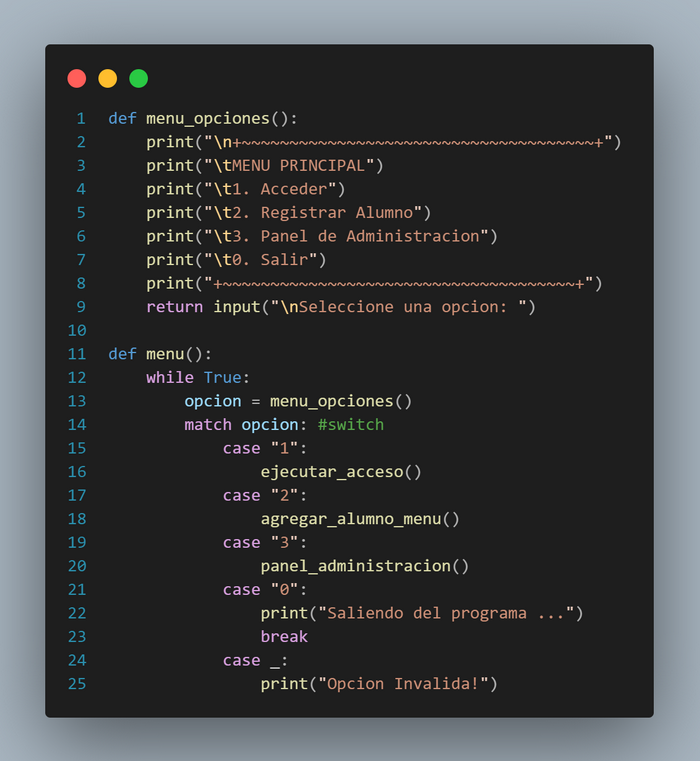
\includegraphics[width=0.8\linewidth]{img/Screenshot from 2025-07-01 07-32-22.png}
\end{figure}

\newpage

\subsection{Opción 1. Acceder}
Esta opción ejecuta el módulo de autenticación mediante la función ejecutar\_acceso(). El flujo comprende la verificación del código a través de la función leer\_qr\_camara, por consiguiente, si el código es verificado se llama a la función verificar\_rostro.

%imagen
\begin{figure}[h]
    \centering
    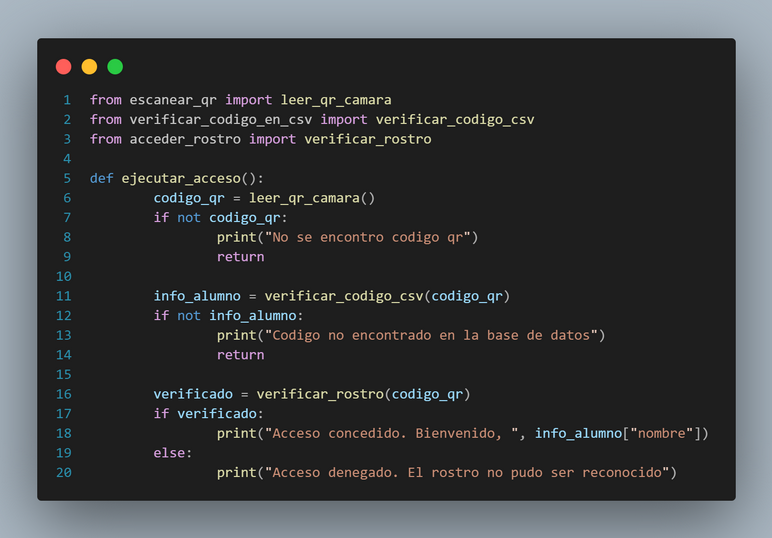
\includegraphics[width=0.8\linewidth]{img/Screenshot from 2025-07-01 07-32-39.png}
\end{figure}

\newpage

\subsubsection{Escanear QR}
Utiliza la librería zxingcpp para detectar códigos QR en tiempo real mediante la cámara web, se captura frames continuamente hasta encontrar un código válido o hasta que el usuario presione ESC. Al finalizar retorna el texto contenido en el QR (código de estudiante) o None si no se detecta.

%imagen
\begin{figure}[h]
    \centering
    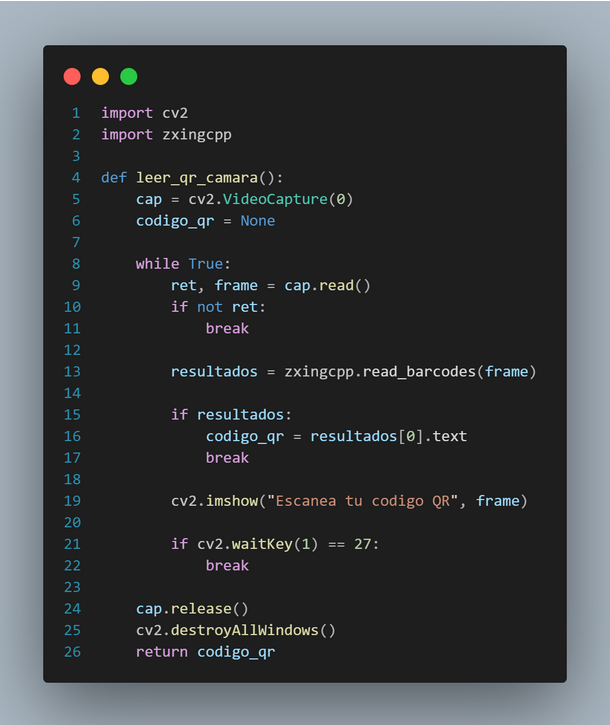
\includegraphics[width=0.8\linewidth]{img/Screenshot from 2025-07-01 07-32-53.png}
\end{figure}

\subsubsection{Verificar código}
Busca el código escaneado en el archivo CSV (alumnos.csv), si este existe, retorna un diccionario con los datos del alumno (nombre, carrera); de lo contrario, retorna None; es decir, si falla, notifica la ausencia del modelo y aborta el proceso.

%imagen
\begin{figure}[h]
    \centering
    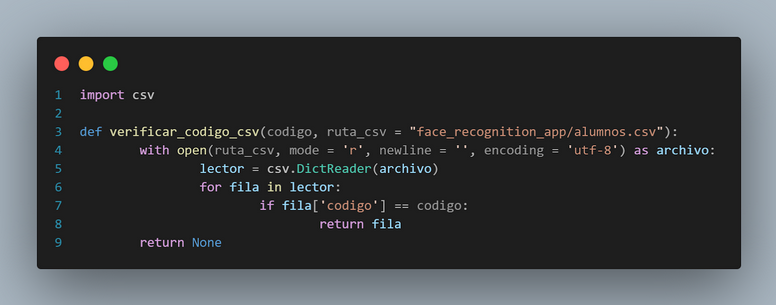
\includegraphics[width=0.8\linewidth]{img/Screenshot from 2025-07-01 07-33-01.png}
\end{figure}

\subsubsection{Reconocimiento facial}
La función comienza creando y cargando un modelo de reconocimiento facial correspondiente al código (modelo\_lbph\_[codigo].yml). Se inicia la captura de video desde la cámara predeterminada y carga un clasificador en cascada pre entrenado para la detección de rostros.

\begin{figure}[h]
    \centering
    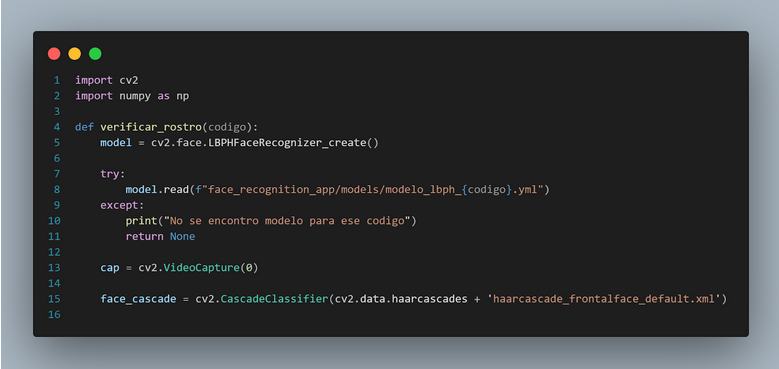
\includegraphics[width=0.8\linewidth]{img/Screenshot from 2025-07-01 07-33-09.png}
\end{figure}

\newpage

Iniciamos un bucle para capturar los frames y convertirlo a escala de grises. Los rostros detectados se almacenan en la variable faces como una lista de coordenadas (x, y, w, h) que representan la posición y el tamaño de cada rostro detectado, se redimensiona las detecciones a 200x200 píxeles (mismo tamaño usado en entrenamiento). Compara el rostro capturado con el modelo mediante el algoritmo LBPH: Umbral de confianza en la cual los valores < 40 indican coincidencia válida (menor valor = mayor similitud). Muestra un rectángulo verde y el nivel de confianza si la verificación es exitosa, o rojo si falla.

%imagen
\begin{figure}[h]
    \centering
    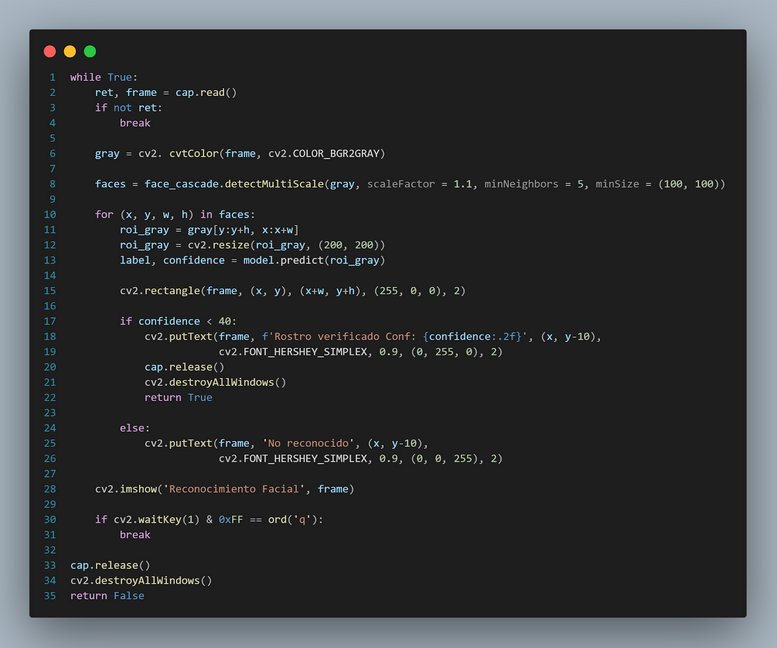
\includegraphics[width=0.8\linewidth]{img/Screenshot from 2025-07-01 07-33-19.png}
\end{figure}

\newpage

\subsection{Opción 2. Registrar alumno}
Esta opción ejecuta el módulo de autenticación mediante la función agregar\_alumno\_menu(). El módulo de registro se compone de tres componentes principales que trabajan en conjunto: captura de datos (validación de código, ingreso de nombre y carrera), generación de QR (Creación del identificador visual único) y registro facial: implementado en dos variantes (cámara en vivo/video pregrabado).

%imagen
\begin{figure}[h]
    \centering
    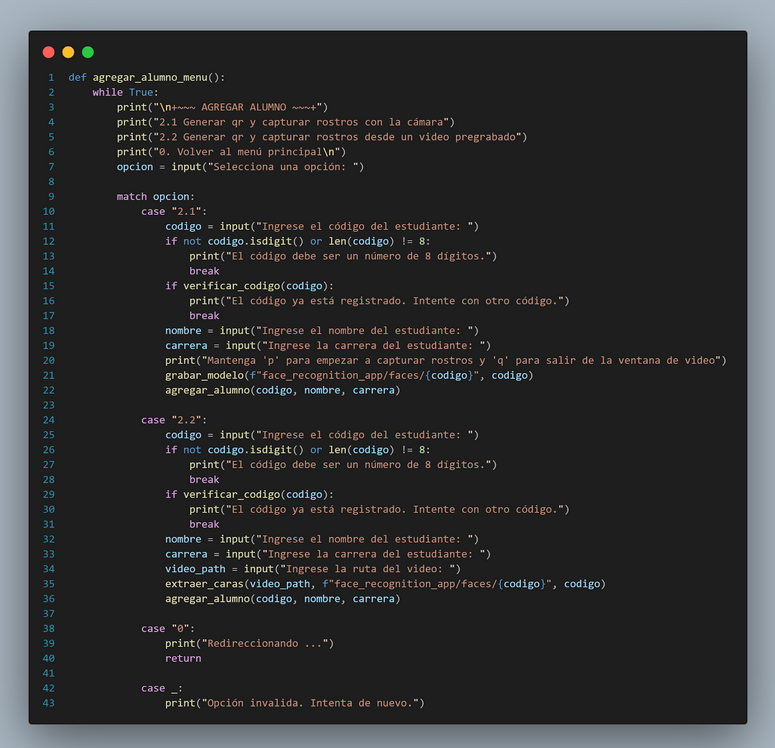
\includegraphics[width=0.8\linewidth]{img/Screenshot from 2025-07-01 07-33-35.png}
\end{figure}

\newpage

\subsubsection{Validación de datos}
Se verifica que el código sea un número entero de 8 dígitos y a través de la función verificar\_codigo() se abre el archivo csv con la información de los estudiantes retornando true si el código ya existe esto hace que sea completamente único en la base de datos.

%imagen
\begin{figure}[h]
    \centering
    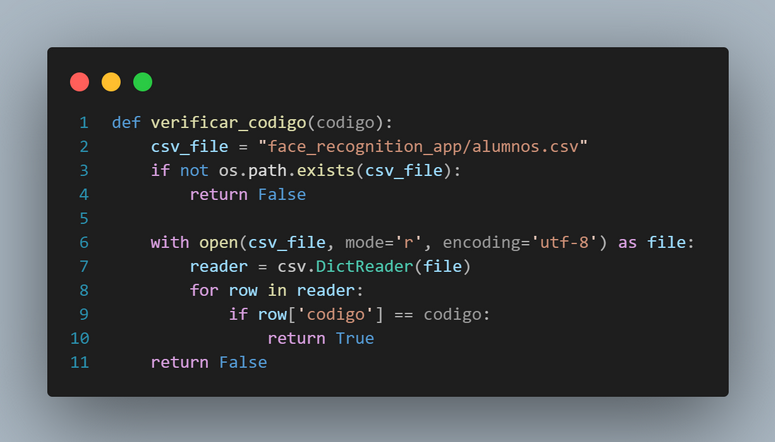
\includegraphics[width=0.8\linewidth]{img/Screenshot from 2025-07-01 07-33-45.png}
\end{figure}

\newpage

\subsubsection{Almacenamiento de Datos}
Una vez validado se llama a la funcion agregar\_alumno() que contiene las rutas donde se guardaran los datos y llama a las funciones anidadas que serviran para continuar con el flujo del programa.

%imagen
\begin{figure}[h]
    \centering
    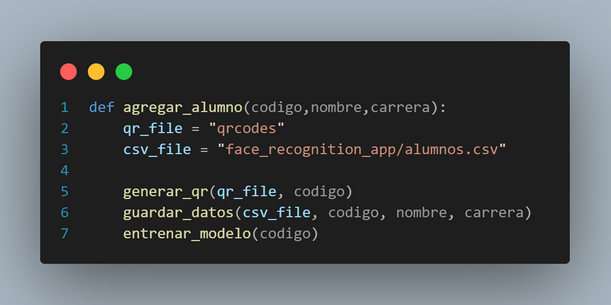
\includegraphics[width=0.8\linewidth]{img/Screenshot from 2025-07-01 07-33-55.png}
\end{figure}

\newpage

Esta información se almacena en un archivo CSV que funciona como la base de datos central del sistema, con manejo de casos especiales crea el archivo con cabeceras si no existe y añade nuevos registros en modo append.

%imagen
%imagen
\begin{figure}[h]
    \centering
    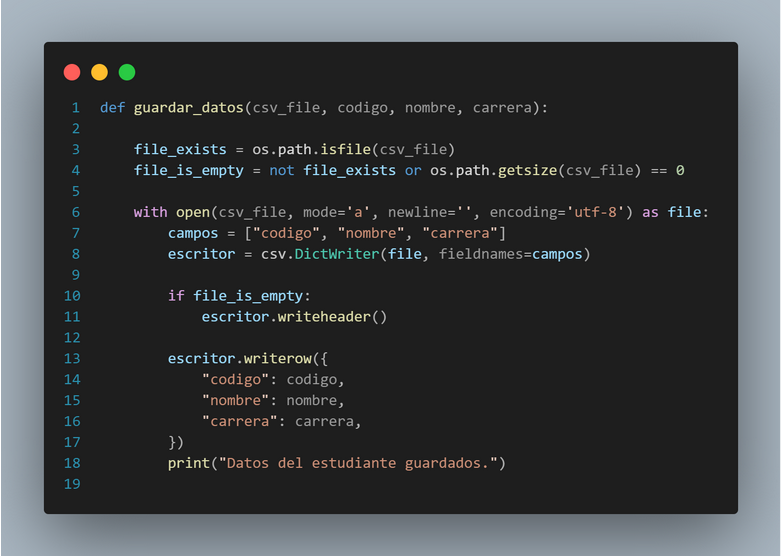
\includegraphics[width=0.8\linewidth]{img/Screenshot from 2025-07-01 07-34-02.png}
\end{figure}

Simultáneamente, se genera un código QR único vinculado al código del estudiante, que servirá como su credencial digital para futuros accesos. Donde también se configura parámetros del QR (versión 1, corrección de errores L).

%imagen
%imagen
\begin{figure}[h]
    \centering
    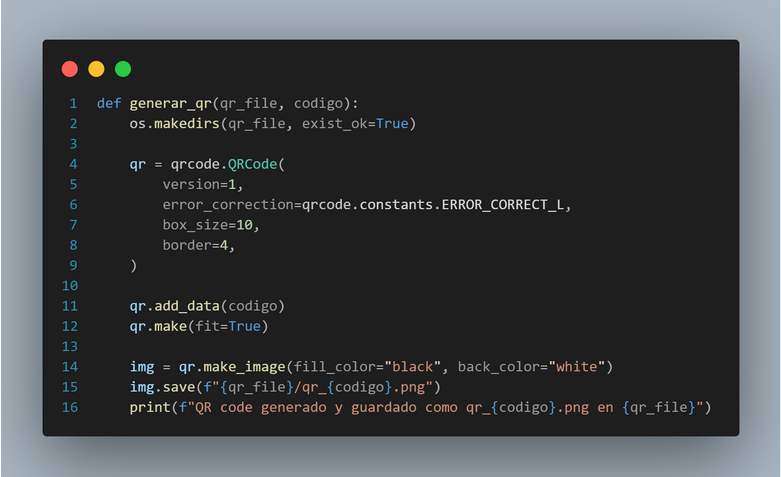
\includegraphics[width=0.8\linewidth]{img/Screenshot from 2025-07-01 07-34-10.png}
\end{figure}

\newpage

\subsubsection{Registro por Cámara}
Esta opción ofrece una alternativa de captura en tiempo real mediante la cámara web. Se muestra el video en tiempo real y se transforma el frame en escala de grises. Después de abrir el video, el código verifica si se pudo abrir correctamente.
Usamos cv2.VideoCapture para capturar videos desde un archivo o una fuente de video en tiempo real, permite leer cuadros (frames) del video uno por uno para su procesamiento. Al mantener presionado la tecla ’p’ activa la captura de rostros y cuando se mantiene la tecla ’q’ finaliza el proceso deteniendo la captura de video. Cada imagen capturada se guarda automáticamente en una carpeta específica para ese alumno.

%imagen
\begin{figure}[h]
    \centering
    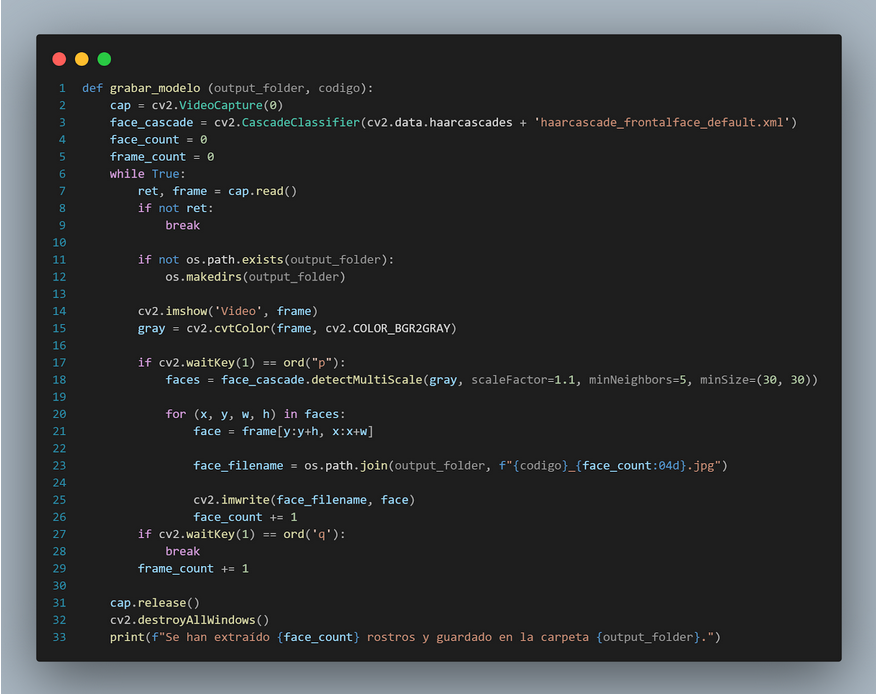
\includegraphics[width=0.8\linewidth]{img/Screenshot from 2025-07-01 07-34-25.png}
\end{figure}

\newpage

\subsubsection{Registro por video}
Para situaciones donde no es posible realizar la captura en directo, el sistema permite cargar un video existente del alumno. Aunque comparte algunos elementos técnicos con la primera opción, como el uso de un
bucle para leer los frames y el uso del clasificador Haar Cascade, su implementación presenta diferencias clave en el flujo de trabajo y la interacción con el usuario.

%imagen
%imagen
\begin{figure}[h]
    \centering
    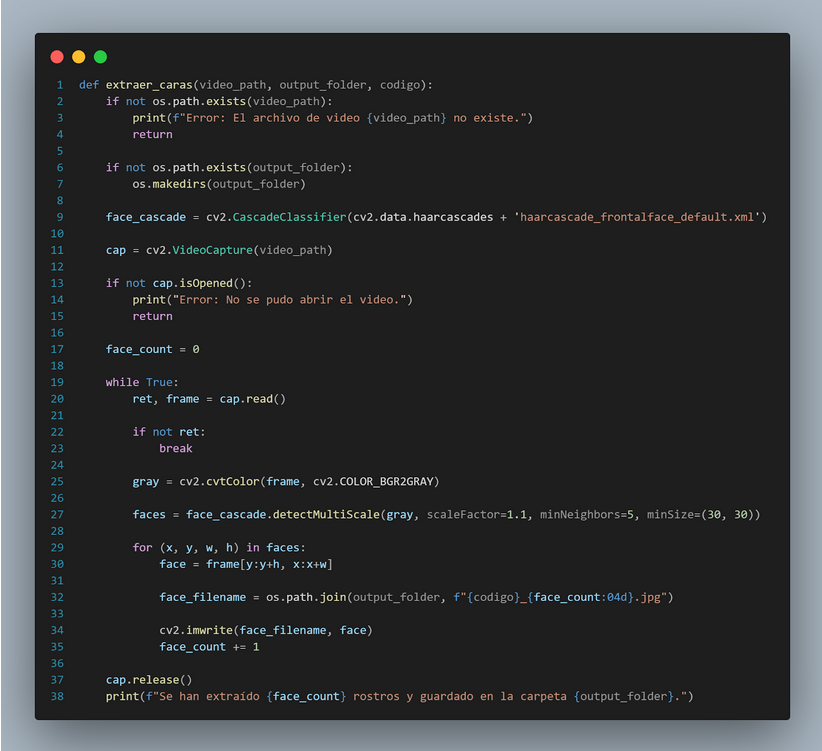
\includegraphics[width=0.8\linewidth]{img/Screenshot from 2025-07-01 07-34-35.png}
\end{figure}

\newpage

\subsubsection{Entrenamiento}
Una vez completada la captura de imágenes faciales (ya sea por cámara o video) se utiliza el algoritmo LBPH (Local Binary Patterns Histograms) para analizar todas las imágenes capturadas y crear un modelo matemático único que representa los rasgos faciales del alumno se lee todas las fotos del directorio del alumno convirtiendo las imágenes a escala de grises y redimensiona a 200x200 píxeles. Este modelo se guarda en un archivo especializado que luego será consultado cada vez que el alumno intente acceder al sistema.

%imagen
\begin{figure}[h]
    \centering
    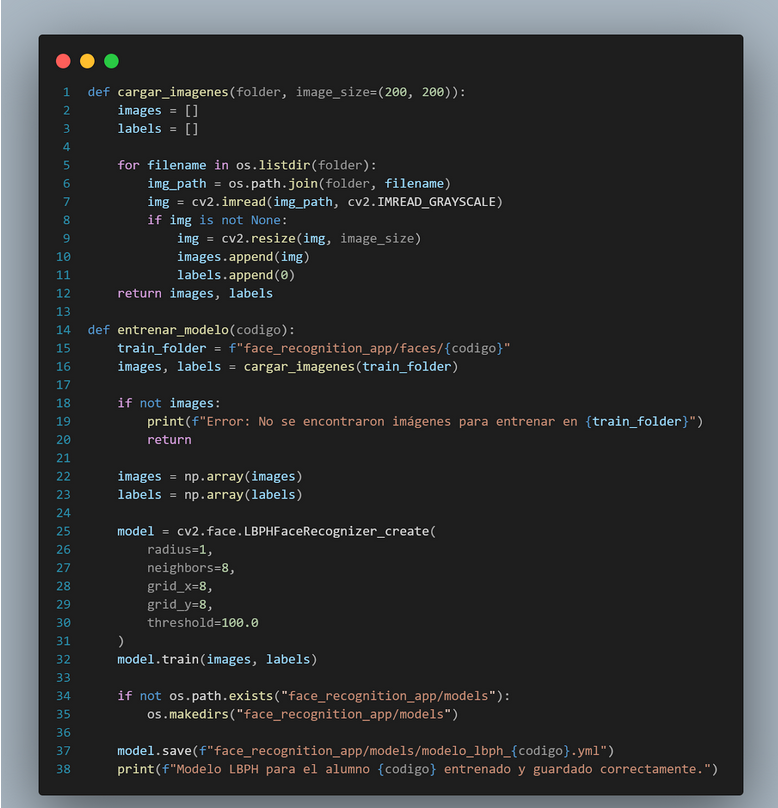
\includegraphics[width=0.8\linewidth]{img/Screenshot from 2025-07-01 07-34-45.png}
\end{figure}

\newpage

\subsection{Opción 3. Panel de administración}
\subsubsection{Importaciones y configuración inicial}

%imagen
\begin{figure}[h]
    \centering
    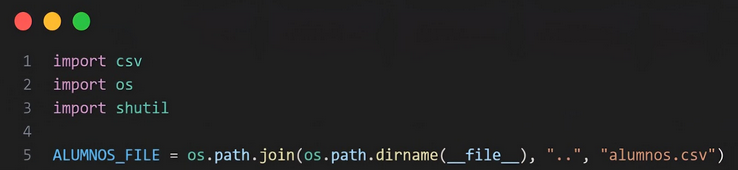
\includegraphics[width=0.8\linewidth]{img/Screenshot from 2025-07-01 07-34-55.png}
\end{figure}

\paragraph{1.1. Importación de librerías necesarias}
\begin{itemize}
    \item \texttt{csv} para manejar archivos CSV.
    \item \texttt{os} para operaciones del sistema operativo.
    \item \texttt{shutil} para operaciones avanzadas de archivos.
\end{itemize}

\paragraph{1.2. Define la ubicación del archivo de alumnos}
\begin{itemize}
    \item Se crea una ruta relativa al archivo \texttt{alumnos.csv} que está en el directorio padre:\\
    \texttt{os.path.join(os.path.dirname(\_\_file\_\_), "..")}
\end{itemize}

\subsubsection{Función: \texttt{mostrar\_alumnos()}}

%imagen
\begin{figure}[h]
    \centering
    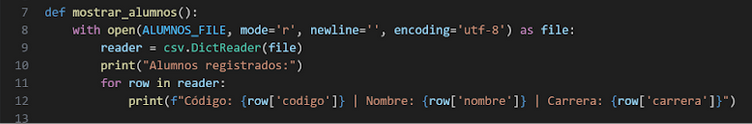
\includegraphics[width=0.8\linewidth]{img/Screenshot from 2025-07-01 07-35-03.png}
\end{figure}

\paragraph{2.1. Apertura del archivo CSV}
\begin{itemize}
    \item Se usa \texttt{with open(...)} para abrir el archivo \texttt{alumnos.csv} en modo lectura (\texttt{mode='r'}) con codificación UTF-8.
    \item El parámetro \texttt{encoding='utf-8'} garantiza que se lean correctamente los caracteres especiales.
    \item \texttt{newline=''} evita problemas con saltos de línea adicionales en algunos sistemas.
\end{itemize}

\paragraph{2.2. Lectura del contenido con \texttt{DictReader}}
\begin{itemize}
    \item \texttt{csv.DictReader(file)} permite leer el archivo como una lista de diccionarios, donde las claves son los nombres de las columnas.
    \item Esto facilita el acceso a los valores por nombre de campo (por ejemplo: \texttt{row['nombre']}).
\end{itemize}

\paragraph{2.3. Impresión de los datos de los alumnos}
\begin{itemize}
    \item Se recorre cada fila del archivo con un bucle \texttt{for row in reader:}
    \item Se imprime cada registro con formato, mostrando el código, nombre y carrera del alumno.
\end{itemize}

\subsubsection{Función: \texttt{borrar\_alumno(codigo)}}

\paragraph{3.1. Buscar y filtrar el alumno}

%imagen
\begin{figure}[h]
    \centering
    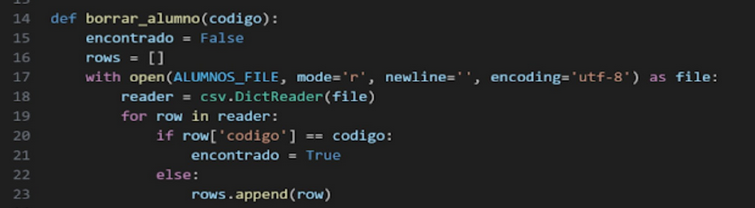
\includegraphics[width=0.8\linewidth]{img/Screenshot from 2025-07-01 07-35-12.png}
\end{figure}

\begin{itemize}
    \item Inicializa variables para rastrear si se encontró el alumno.
    \item Lee el archivo CSV y recorre cada registro.
    \item Si encuentra el código, marca \texttt{encontrado} como \texttt{True}.
    \item Si no es el alumno a borrar, lo agrega a la lista \texttt{rows}.
\end{itemize}


\paragraph{3.2. Verificación y reescritura}

\begin{itemize}
    \item Si no encontró el alumno, muestra mensaje y termina.
    \item Si lo encontró, reescribe el archivo CSV con todos los alumnos excepto el borrado.
    \item Mantiene la estructura original con cabeceras.
\end{itemize}

%imagen
\begin{figure}[h]
    \centering
    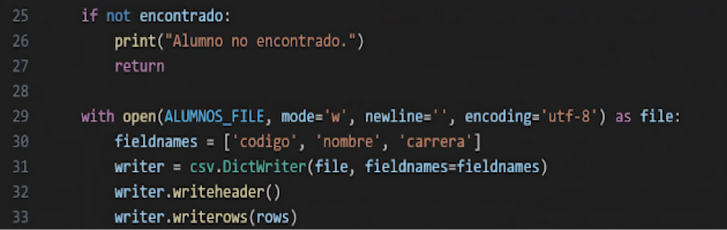
\includegraphics[width=0.8\linewidth]{img/Screenshot from 2025-07-01 07-35-19.png}
\end{figure}

\paragraph{3.3. Eliminación de archivos asociados}

\begin{itemize}
    \item Construye la ruta a la carpeta de caras del alumno.
    \item Si existe, la elimina recursivamente con \texttt{shutil.rmtree()}.
\end{itemize}

%imagen
\begin{figure}[h]
    \centering
    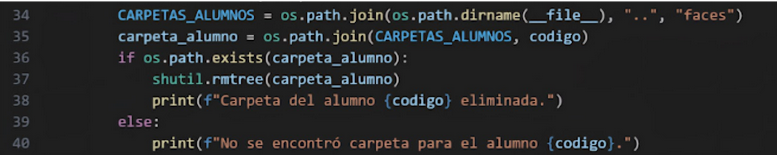
\includegraphics[width=0.8\linewidth]{img/Screenshot from 2025-07-01 07-35-27.png}
\end{figure}

%imagen
\begin{figure}[h]
    \centering
    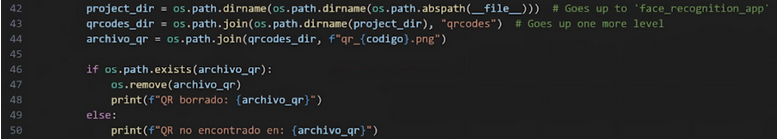
\includegraphics[width=0.8\linewidth]{img/Screenshot from 2025-07-01 07-35-35.png}
\end{figure}


\begin{itemize}
    \item Busca y elimina el archivo QR asociado al alumno.
    \item Busca y elimina el modelo de reconocimiento facial asociado.
    \item Muestra el mensaje final de confirmación.
\end{itemize}

%imagen
\begin{figure}[h]
    \centering
    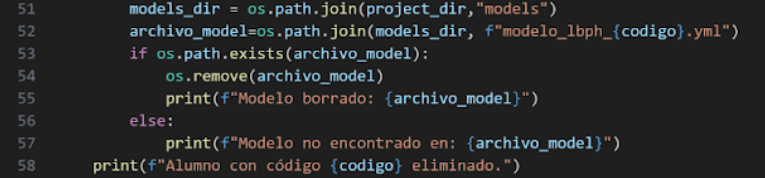
\includegraphics[width=0.8\linewidth]{img/Screenshot from 2025-07-01 07-35-44.png}
\end{figure}

\newpage

\subsubsection{Función: \texttt{editar\_informaci\'on}}

\paragraph{Parte 1: Buscar y modificar}

\begin{itemize}
    \item Inicializa variables para rastrear si se actualizó el alumno.
    \item Lee el archivo CSV y busca el alumno por código.
    \item Si lo encuentra, actualiza nombre y/o carrera según los parámetros.
    \item Agrega todos los registros (modificados o no) a la lista \texttt{rows}.
\end{itemize}

%imagen
\begin{figure}[h]
    \centering
    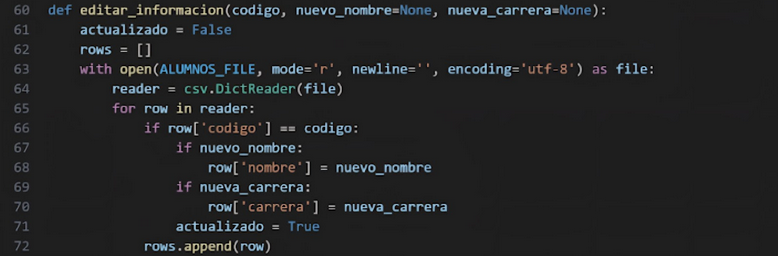
\includegraphics[width=0.8\linewidth]{img/Screenshot from 2025-07-01 07-35-55.png}
\end{figure}

\paragraph{Parte 2: Reescritura del archivo}

\begin{itemize}
    \item Si se realizaron cambios, reescribe el archivo CSV completo.
    \item Si no encontró el alumno, muestra mensaje de error.
\end{itemize}

%imagen
\begin{figure}[h]
    \centering
    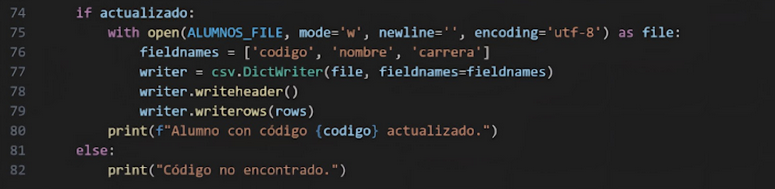
\includegraphics[width=0.8\linewidth]{img/Screenshot from 2025-07-01 07-36-02.png}
\end{figure}

\section{Resultados}

\subsubsection{Flujo de funcionamiento del sistema}

\paragraph{Registro inicial}
Este sistema representa el primer paso al ejecutar el código por primera vez, ya que no existen registros previos de alumnos. El menú principal ofrece la opción de registrar un nuevo alumno (Opción 2), lo que permite comenzar a construir una base de datos de rostros y códigos QR asociados a cada estudiante.

El proceso inicia con la captura facial mediante la cámara en tiempo real (Opción 2.1) o desde un video (Opción 2.2). Al ingresar los datos del alumno (código, nombre y carrera), el sistema realiza las siguientes acciones:

\begin{figure}[h]
    \centering
    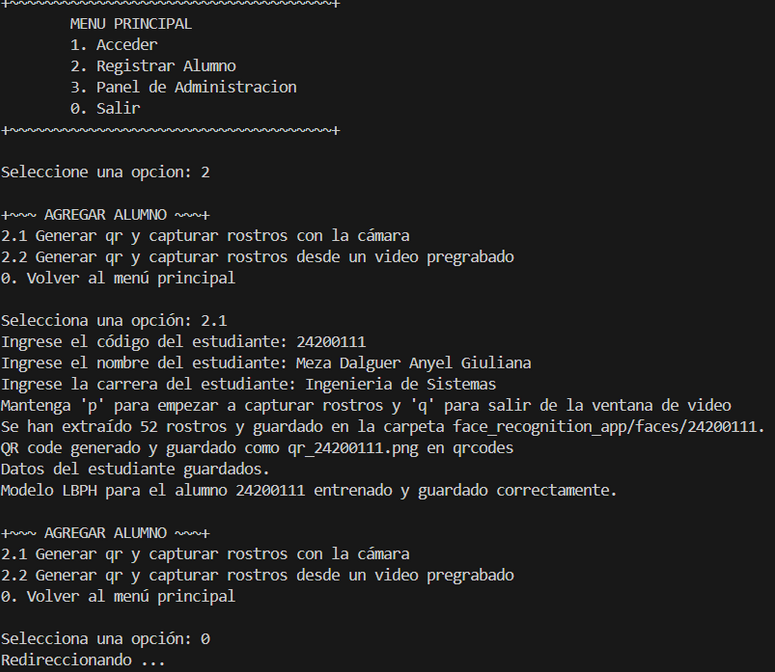
\includegraphics[width=0.8\linewidth]{img/Screenshot from 2025-07-01 08-45-34.png}
\end{figure}

\begin{itemize}
    \item Extrae múltiples imágenes del rostro (ej: 52 capturas) y las guarda en una carpeta dedicada.
    \item Genera un código QR único vinculado al estudiante.
    \item Entrena un modelo de reconocimiento facial (LBPH) con las imágenes obtenidas.
\end{itemize}

Este flujo asegura que, desde la primera ejecución, el sistema pueda almacenar rostros, asociarlos a un identificador y preparar el modelo para futuras verificaciones. Posteriormente, con más registros, el sistema podrá comparar rostros en tiempo real contra la base de datos creada.

La estructura modular del menú permite escalar el sistema añadiendo más funciones, como el acceso de alumnos registrados (Opción 1) o el panel de administración (Opción 3), una vez se hayan cargado datos iniciales.

\begin{figure}[h]
    \centering
    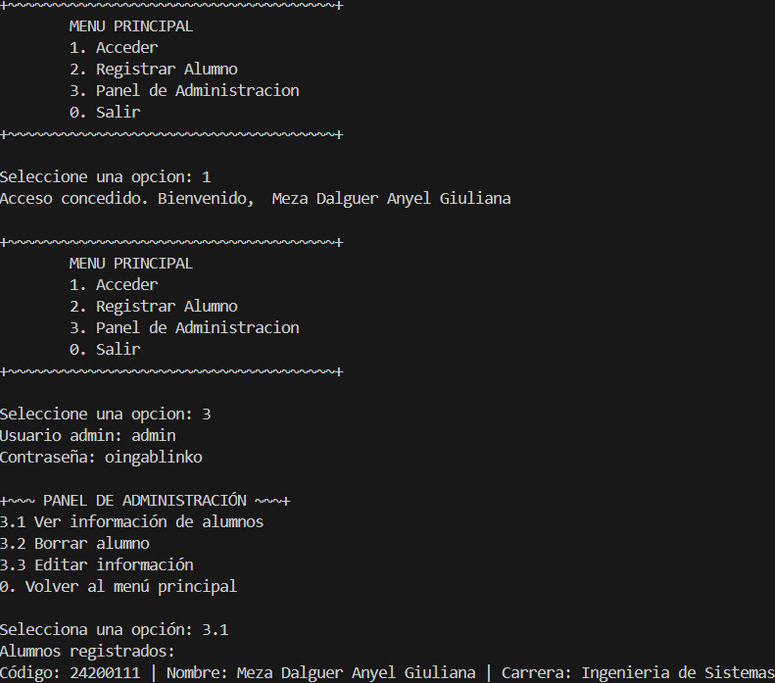
\includegraphics[width=0.8\linewidth]{img/Screenshot from 2025-07-01 08-45-54.png}
\end{figure}

\paragraph{Acceso del alumno (Opción 1)}
Este segmento muestra el proceso de acceso y administración del sistema una vez se han registrado alumnos. El flujo se divide en dos partes clave:

\begin{itemize}
    \item \textbf{Lectura del código QR:} Al seleccionar \textit{Acceder}, el sistema activa la cámara para escanear el código QR del alumno previamente generado (ej: \texttt{qr\_24200111.png}). El QR contiene el código único del estudiante (ej: \texttt{24200111}).
    \item \textbf{Verificación facial en tiempo real:} Tras leer el QR, la cámara se reactiva para capturar el rostro del usuario y lo compara con el modelo LBPH entrenado durante el registro. Si coincide, muestra el mensaje: \texttt{"Acceso concedido. Bienvenido, [Nombre del alumno]"} (ej: Meza Dalguer Anyel Giuliana).
\end{itemize}

\paragraph{Panel de administración (Opción 3)}

\textbf{Autenticación:}
\begin{itemize}
    \item Requiere credenciales de administrador (ej: usuario: \texttt{admin}, contraseña: \texttt{oingablinko}).
\end{itemize}

\textbf{Gestión de alumnos:}
\begin{itemize}
    \item \textbf{Opción 3.1:} Muestra la lista de alumnos registrados con sus datos (código, nombre, carrera).
\end{itemize}

\paragraph{Integración de tecnologías}
\begin{itemize}
    \item \textbf{OpenCV:} Para la captura de video, detección de QR y reconocimiento facial.
    \item \textbf{LBPH (Local Binary Patterns Histograms):} Algoritmo que verifica la identidad del alumno comparando los rostros capturados con los almacenados.
    \item \textbf{Base de datos implícita:} Los datos se guardan en archivos (carpetas de rostros, QR) y posiblemente en un archivo CSV o JSON para la información administrativa.
\end{itemize}

\paragraph{Contexto de uso}
\begin{itemize}
    \item \textbf{Primer registro → Acceso:} El sistema evoluciona desde el registro inicial (sin datos) hasta permitir el acceso seguro mediante autenticación multimodal (QR + rostro).
    \item \textbf{Escalabilidad:} El panel de administración sugiere que el sistema está diseñado para manejar múltiples alumnos y permitir mantenimiento (ej: en entornos educativos).
\end{itemize}

\begin{figure}[h]
    \centering
    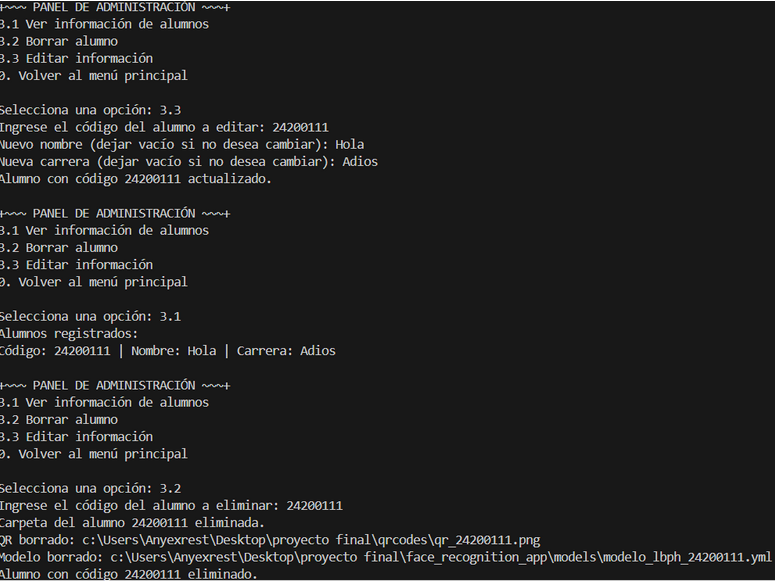
\includegraphics[width=0.8\linewidth]{img/Screenshot from 2025-07-01 08-46-17.png}
\end{figure}

\subsubsection{Edición y eliminación de registros de alumnos}

Este segmento completa el flujo del sistema mostrando las funciones avanzadas de administración, específicamente la edición de datos y la eliminación de registros de alumnos.

\paragraph{Edición de información del alumno (Opción 3.3)}
\begin{itemize}
    \item \textbf{Selección del alumno:} El administrador ingresa el código del alumno a modificar (ej: \texttt{24200111}).
    \item \textbf{Actualización flexible:} Permite cambiar nombre y carrera de forma independiente (ej: nombre → \texttt{"Hola"}, carrera → \texttt{"Adios"}). Los campos vacíos mantienen los valores anteriores.
    \item \textbf{Confirmación:} El sistema actualiza los datos y muestra un mensaje de éxito (\texttt{"Alumno con código 24200111 actualizado"}).
\end{itemize}

\paragraph{Eliminación de alumno (Opción 3.2)}
\begin{itemize}
    \item \textbf{Proceso completo de borrado:}
    \begin{itemize}
        \item Elimina la carpeta de rostros asociada al alumno (ej: \texttt{face\_recognition\_app/faces/24200111}).
        \item Borra el código QR del alumno (ruta: \texttt{.../qrcodes/qr\_24200111.png}).
        \item Remueve el modelo entrenado (ej: \texttt{modelo\_lbph\_24200111.qml}).
    \end{itemize}
    \item \textbf{Confirmación:} Mensaje detallado con las rutas eliminadas y confirmación final (\texttt{"Alumno con código 24200111 eliminado"}).
\end{itemize}

\paragraph{Tecnologías y estructura implicadas}
\begin{itemize}
    \item \textbf{Gestión de archivos:} Eliminación de carpetas (rostros), imágenes (QR) y modelos (LBPH) mediante operaciones del sistema.
    \item \textbf{Persistencia de datos:} Los cambios se reflejan inmediatamente en la lista de alumnos (visible al usar Opción 3.1).
    \item \textbf{Seguridad:} Solo accesible tras autenticación como administrador.
\end{itemize}

\paragraph{Contexto y escalabilidad}
\begin{itemize}
    \item \textbf{Mantenimiento eficiente:} Permite corregir errores (ej: nombres mal escritos) o dar de baja alumnos que ya no requieran acceso.
    \item \textbf{Integridad del sistema:} Al eliminar un alumno, se liberan recursos (espacio en disco) y se evitan conflictos en el reconocimiento facial.
\end{itemize}

Estas funciones cierran el ciclo de vida de un alumno en el sistema, demostrando su capacidad para manejar registros dinámicos en entornos educativos o laborales.

\textbf{Resumen del ciclo:}
\begin{center}
\texttt{1. Registrar alumno → 2. Acceder con QR + rostro → 3. Editar/Eliminar (admin) → 4. Ver cambios en tiempo real}
\end{center}

\begin{figure}[h]
    \centering
    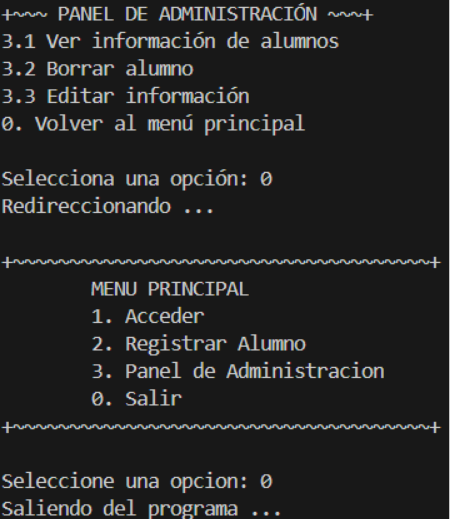
\includegraphics[width=0.8\linewidth]{img/Screenshot from 2025-07-01 08-46-33.png}
\end{figure}

\subsubsection{Flujo de salida del sistema}

Este segmento muestra el flujo de salida del sistema, tanto desde el Panel de Administración como desde el Menú Principal, cerrando el programa de manera ordenada.

\paragraph{Volver al Menú Principal (Opción 0 en Panel de Administración)}
\begin{itemize}
    \item \textbf{Redirección:} Al seleccionar la opción 0 en el Panel de Administración, el sistema retorna al Menú Principal sin cerrarse, permitiendo continuar con otras operaciones.
\end{itemize}

\paragraph{Salir del Programa (Opción 0 en Menú Principal)}
\begin{itemize}
    \item \textbf{Finalización controlada:} Al elegir 0 en el Menú Principal, el sistema muestra el mensaje \texttt{"Saliendo del programa ..."} y termina su ejecución de manera segura.
\end{itemize}

\paragraph{Tecnologías y estructura implicadas}
\begin{itemize}
    \item \textbf{Manejo de bucles:} El sistema utiliza un bucle principal (\texttt{while True}) que se rompe únicamente al seleccionar la opción de salida.
    \item \textbf{Modularidad:} Cada menú (Principal, Administración) funciona como un módulo independiente, facilitando la navegación y el cierre controlado.
\end{itemize}

\paragraph{Contexto y usabilidad}
\begin{itemize}
    \item \textbf{Experiencia de usuario:} La opción 0 actúa como estándar para salir/volver en todos los menús, haciendo el sistema intuitivo.
\end{itemize}

%Conclusiones y recomendaciones
\section{Conclusiones y recomendaciones}

El desarrollo del sistema de reconocimiento facial ha permitido cumplir con los objetivos planteados y demostrar su viabilidad técnica y práctica. A continuación, se destacan los principales logros obtenidos:

\subsection*{Implementación funcional del sistema}
\begin{itemize}
    \item El sistema de registro del estudiante, generación de código QR y modelo de reconocimiento facial funciona correctamente y es fácil de comprender gracias a una interfaz de usuario agradable.
    \item El sistema permite dos métodos de registro (carga de video y grabación en tiempo real), lo que lo hace versátil para diferentes escenarios de uso.
\end{itemize}

\subsection*{Optimización del procesamiento de imágenes}
\begin{itemize}
    \item Se implementó con éxito el preprocesamiento de imágenes (conversión a escala de grises, redimensionamiento y detección de rostros), mejorando la eficiencia del modelo y reduciendo el consumo de recursos computacionales.
    \item El uso del clasificador Haar Cascade y el algoritmo Eigenfaces demostró ser efectivo para un reconocimiento preciso en condiciones controladas.
\end{itemize}

\subsection*{Integración de un menú interactivo}
\begin{itemize}
    \item Se diseñó una interfaz de usuario intuitiva mediante un menú en consola que guía al usuario a través de las funciones principales:
    \begin{itemize}
        \item Registro de nuevos rostros.
        \item Verificación de acceso.
        \item Panel de administración.
    \end{itemize}
\end{itemize}

\subsection*{Validación del modelo}
\begin{itemize}
    \item El sistema fue probado con éxito en un entorno simulado, logrando:
    \begin{itemize}
        \item Identificación correcta de rostros previamente registrados.
        \item Generación de un nivel de confianza para cada predicción, permitiendo filtrar reconocimientos ambiguos.
    \end{itemize}
    \item Sin embargo, se observó que el rendimiento disminuye en entornos con iluminación variable (por ejemplo, sombras o luz natural cambiante), lo que sugiere la necesidad de mejorar el preprocesamiento de imágenes o adoptar modelos más robustos, como los basados en \textit{Deep Learning}, en futuras iteraciones.
\end{itemize}

\subsection*{Contribución a la automatización y seguridad}
\begin{itemize}
    \item El proyecto sentó las bases para un sistema escalable que podría:
    \begin{itemize}
        \item Reemplazar métodos tradicionales de identificación (por ejemplo, carnets físicos).
        \item Reducir los tiempos de verificación en accesos institucionales.
        \item Integrarse con bases de datos para aplicaciones de control de asistencia o seguridad.
    \end{itemize}
\end{itemize}

\subsection*{Trabajo colaborativo y aprendizaje técnico}
\begin{itemize}
    \item Se consolidaron habilidades en Python, OpenCV y \textit{machine learning} aplicado al procesamiento de imágenes.
    \item El desarrollo en equipo permitió abordar desafíos técnicos y mejorar la solución mediante iteraciones.
\end{itemize}

%Bibliografía
\section{Bibliografía}
S. M. Metev, La librería Numpy, 2nd ed., R. M. Osgood, Jr., Ed. Berlin, Germany: Springer- Verlag, 2008. Disponible: https://aprendeconalf.es/docencia/python/manual/numpy 


M. Khan, S. Chakraborty, R. Astya and S. Khepra, "Face Detection and Recognition Using OpenCV," 2019 International Conference on Computing, Communication, and Intelligent Systems (ICCCIS), Greater Noida, India, 2019, pp. 116-119, doi: 10.1109/ICCCIS48478.2019.8974493


Ahonen, T., Hadid, A., \& Pietikäinen, M. (2006). Face description with local binary patterns: Application to face recognition. IEEE Transactions on Pattern Analysis and Machine Intelligence, 28(12), 2037–2041. https://doi.org/10.1109/TPAMI.2006.244


Almeida, J., \& Silva, C. (2021). Optimized facial recognition based on grayscale conversion and low-resolution training. Journal of Artificial Intelligence and Data Mining, 9(2), 45-54. 

Kumar, P., \& Raj, S. (2022). Real-time face detection using Haar cascade classifier and OpenCV. International Journal of Computer Applications, 184(27), 15–20. 

Metev, S. M. (2008). La librería NumPy. In R. M. Osgood, Jr. (Ed.), Manual de Python Científico (2nd ed.). Springer-Verlag.

Sharma, P., Rajpurohit, S. P., \& Jain, A. (2019). Comparative study of various image preprocessing techniques for facial recognition. International Journal of Image, Graphics and Signal Processing, 11(6), 1–10. https://doi.org/10.5815/ijigsp.2019.06.01
Singh, A., \& Nagori, A. (2020). Real-time face recognition system using Local Binary Pattern Histogram (LBPH). Journal of Emerging Technologies and Innovative Research, 7(5), 1452–1458. https://doi.org/10.5281/zenodo.3909938

Turk, M., \& Pentland, A. (1991). Eigenfaces for recognition. Journal of Cognitive Neuroscience, 3(1), 71–86. https://doi.org/10.1162/jocn.1991.3.1.71

Viola, P., \&Jones, M. (2001). Rapid object detection using a boosted cascade of simple features. Proceedings of the 2001 IEEE Computer Society Conference on Computer Vision and Pattern Recognition. https://doi.org/10.1109/CVPR.2001.990517


Zhao, W., Chellappa, R., \& Rosenfeld, A. (2020). Face recognition: A literature survey. ACM Computing Surveys, 35(4), 399–458. https://doi.org/10.1145/954339.954342

}
%Fin del cuerpo del documento
\end{document}